\documentclass[aspectratio=169]{beamer}

\usepackage[T1]{fontenc}
\usepackage[utf8]{inputenc}
\usepackage{lmodern}
\usepackage{microtype}
\usepackage{xcolor}
\usepackage{tikz}
\usetikzlibrary{positioning, arrows.meta}
\usepackage{booktabs}
\usepackage{array}
\usepackage{fontawesome5}

\definecolor{wurgreen}{HTML}{34B233}
\definecolor{darkgreen}{HTML}{1F6B1E}
\definecolor{darknavy}{HTML}{1A1A2E}
\definecolor{midgray}{HTML}{6B7280}
\definecolor{lightgray}{HTML}{F3F4F6}
\definecolor{lightgreen}{HTML}{E8F7E8}
\definecolor{warnred}{HTML}{FEE2E2}
\definecolor{warnborder}{HTML}{EF4444}
\definecolor{bodytext}{HTML}{1F2937}

\usetheme{default}
\usecolortheme{default}
\usefonttheme{professionalfonts}
\setbeamertemplate{navigation symbols}{}
\setbeamertemplate{itemize items}{\textcolor{wurgreen}{\textbullet}}
\setbeamertemplate{itemize subitem}{\textcolor{midgray}{--}}
\setbeamercolor{frametitle}{fg=white, bg=darknavy}
\setbeamerfont{frametitle}{size=\large, series=\bfseries}
\setbeamertemplate{frametitle}{%
  \begin{beamercolorbox}[wd=\paperwidth, ht=1.1cm, dp=0.2cm, leftskip=0.6cm]{frametitle}
    \usebeamerfont{frametitle}\insertframetitle
  \end{beamercolorbox}}
\setbeamercolor{background canvas}{bg=white}
\setbeamercolor{normal text}{fg=bodytext}
\setbeamertemplate{footline}{%
  \begin{beamercolorbox}[wd=\paperwidth, ht=0.4cm, dp=0.15cm]{footline}
    \hspace{0.5cm}\textcolor{midgray}{\tiny Bags, Vectors \& Transformers · Wageningen University \& Research}%
    \hfill\textcolor{midgray}{\tiny \insertframenumber}\hspace{0.4cm}
  \end{beamercolorbox}}

\begin{document}

% ── TITLE SLIDE ──────────────────────────────────────────────────────────────
{
\setbeamertemplate{footline}{}
\begin{frame}[plain]
  \begin{tikzpicture}[remember picture, overlay]
    \fill[darknavy] (current page.south west) rectangle (current page.north east);
    \fill[wurgreen] (current page.south west) rectangle
      ([xshift=0.45cm]current page.north west);
    \node[anchor=west, text=white, font=\huge\bfseries, text width=13cm]
      at ([xshift=1.1cm, yshift=1.2cm]current page.west)
      {Bags, Vectors \& Transformers};
    \node[anchor=west, text=wurgreen, font=\large, text width=12cm]
      at ([xshift=1.1cm, yshift=0.05cm]current page.west)
      {Classic Text Analysis · Day 1, Part 3};
    \node[anchor=west, text=midgray, font=\small, text width=12cm]
      at ([xshift=1.1cm, yshift=-1.5cm]current page.west)
      {Denise J. Roth, PhD Candidate\\
       Strategic Communication Group · Wageningen University \& Research};
  \end{tikzpicture}
\end{frame}
}

% ── SLIDE 1: What is classic CTA? ────────────────────────────────────────────
\begin{frame}{What Do We Mean by ``Classic'' Text Analysis?}
\vspace{0.2cm}
{\small By \textbf{classic} computational text analysis, we mean the family of methods
that treat text as \textbf{counts of words}. The central idea is simple but powerful:
if we can turn documents into \textbf{numbers}, we can compare them, measure them,
and analyze them statistically.}

\bigskip
\begin{columns}[t]
  \column{0.48\textwidth}
  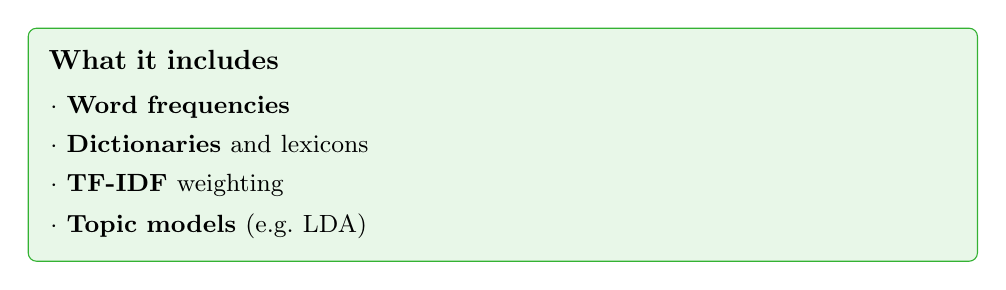
\begin{tikzpicture}
    \node[fill=lightgreen, draw=wurgreen, rounded corners=3pt,
          inner xsep=8pt, inner ysep=8pt, text width=\columnwidth-18pt]{%
      \textbf{What it includes}\\[5pt]
      {\small
      $\cdot$ \textbf{Word frequencies}\\[3pt]
      $\cdot$ \textbf{Dictionaries} and lexicons\\[3pt]
      $\cdot$ \textbf{TF-IDF} weighting\\[3pt]
      $\cdot$ \textbf{Topic models} (e.g.\ LDA)}};
  \end{tikzpicture}

  \column{0.48\textwidth}
  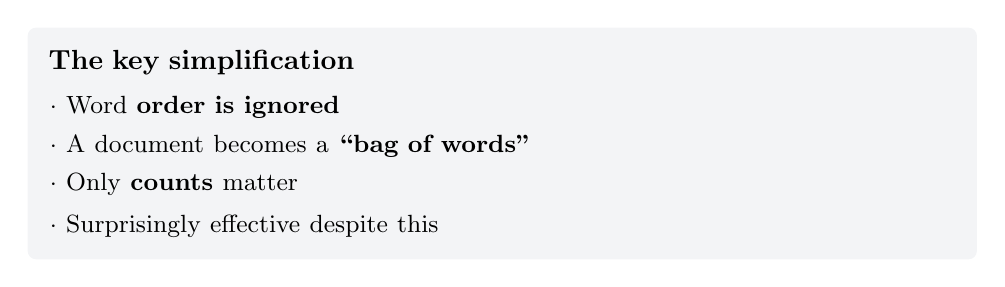
\begin{tikzpicture}
    \node[fill=lightgray, rounded corners=3pt,
          inner xsep=8pt, inner ysep=8pt, text width=\columnwidth-18pt]{%
      \textbf{The key simplification}\\[5pt]
      {\small
      $\cdot$ Word \textbf{order is ignored}\\[3pt]
      $\cdot$ A document becomes a \textbf{``bag of words''}\\[3pt]
      $\cdot$ Only \textbf{counts} matter\\[3pt]
      $\cdot$ Surprisingly effective despite this}};
  \end{tikzpicture}
\end{columns}
\end{frame}

% ── SLIDE 2: A little history ────────────────────────────────────────────────
\begin{frame}{A Little History}
\vspace{0.3cm}
\begin{itemize}\setlength\itemsep{9pt}
  \item[\textcolor{wurgreen}{\faHistory}]
    \textbf{1940s--50s:} early word-counting in the humanities ---
    concordances, authorship studies (who \textit{really} wrote this text?)
  \item[\textcolor{wurgreen}{\faHistory}]
    \textbf{1960s:} \textbf{content analysis} formalized in the social sciences;
    the General Inquirer, one of the first computer-assisted text systems
  \item[\textcolor{wurgreen}{\faHistory}]
    \textbf{1970s--80s:} \textbf{information retrieval} matures ---
    TF-IDF and the vector space model, driven by the need to search documents
  \item[\textcolor{wurgreen}{\faHistory}]
    \textbf{2000s:} \textbf{topic modeling} (LDA, 2003) makes large-scale
    thematic analysis accessible
  \item[\textcolor{wurgreen}{\faHistory}]
    \textbf{2010s onward:} the field shifts toward \textbf{embeddings} and
    \textbf{neural methods} --- but the classic tools remain everywhere
\end{itemize}
\end{frame}

% ── SLIDE 3: Text as data ────────────────────────────────────────────────────
\begin{frame}{The Core Idea: Text as Data}
\vspace{0.4cm}
\begin{center}
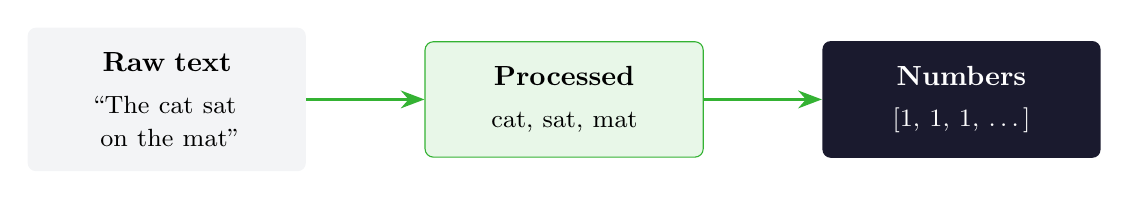
\begin{tikzpicture}[node distance=1.2cm]
  \node[fill=lightgray, rounded corners=3pt, inner sep=9pt, text width=2.9cm, align=center] (raw)
    {\textbf{Raw text}\\[3pt]{\small ``The cat sat on the mat''}};
  \node[fill=lightgreen, draw=wurgreen, rounded corners=3pt, inner sep=9pt,
        text width=2.9cm, align=center, right=1.5cm of raw] (proc)
    {\textbf{Processed}\\[3pt]{\small cat, sat, mat}};
  \node[fill=darknavy, rounded corners=3pt, inner sep=9pt,
        text width=2.9cm, align=center, right=1.5cm of proc] (num)
    {\textcolor{white}{\textbf{Numbers}}\\[3pt]{\small\textcolor{white}{[1, 1, 1, \ldots]}}};
  \draw[-{Stealth[length=3mm]}, wurgreen, line width=1.2pt] (raw) -- (proc);
  \draw[-{Stealth[length=3mm]}, wurgreen, line width=1.2pt] (proc) -- (num);
\end{tikzpicture}
\end{center}

\bigskip
{\small The whole enterprise rests on one move: \textbf{transforming text into a
numerical representation} a computer can work with. Everything else --- counting,
weighting, modeling --- builds on this. The rest of this session is about the
vocabulary you need to understand that move.}
\end{frame}

% ── SLIDE 4: Prerequisites - corpus and documents ────────────────────────────
\begin{frame}{Prerequisite Concepts (1): Corpus \& Documents}
\vspace{0.3cm}
\begin{columns}[t]
  \column{0.48\textwidth}
  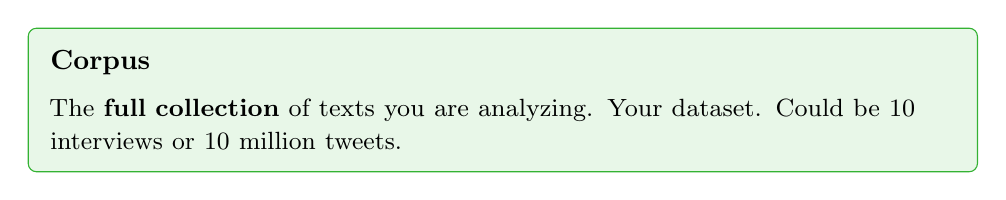
\begin{tikzpicture}
    \node[fill=lightgreen, draw=wurgreen, rounded corners=3pt,
          inner xsep=8pt, inner ysep=8pt, text width=\columnwidth-18pt]{%
      \textbf{Corpus}\\[5pt]
      {\small The \textbf{full collection} of texts you are analyzing.
      Your dataset. Could be 10 interviews or 10 million tweets.}};
  \end{tikzpicture}

  \column{0.48\textwidth}
  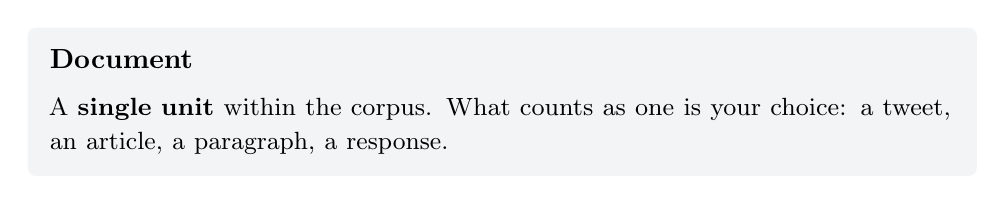
\begin{tikzpicture}
    \node[fill=lightgray, rounded corners=3pt,
          inner xsep=8pt, inner ysep=8pt, text width=\columnwidth-18pt]{%
      \textbf{Document}\\[5pt]
      {\small A \textbf{single unit} within the corpus. What counts as one
      is your choice: a tweet, an article, a paragraph, a response.}};
  \end{tikzpicture}
\end{columns}

\bigskip
{\small\textcolor{midgray}{\textit{Deciding what your ``document'' is matters ---
it shapes everything downstream. One survey response? One sentence? One respondent's
full answer set? There is no universally right answer, only what fits your question.}}}
\end{frame}

% ── SLIDE 5: Prerequisites - tokens, types, vocabulary ───────────────────────
\begin{frame}{Prerequisite Concepts (2): Tokens, Types, Vocabulary}
\vspace{0.3cm}
\begin{itemize}\setlength\itemsep{10pt}
  \item \textbf{Token:} a single occurrence of a word in a text.
        ``the cat sat on the mat'' has \textbf{6 tokens}.
  \item \textbf{Type:} a distinct word. That same sentence has \textbf{5 types}
        (``the'' appears twice but counts once).
  \item \textbf{Vocabulary:} the \textbf{set of all types} across your whole corpus ---
        the columns of the matrix we are about to build.
\end{itemize}

\bigskip
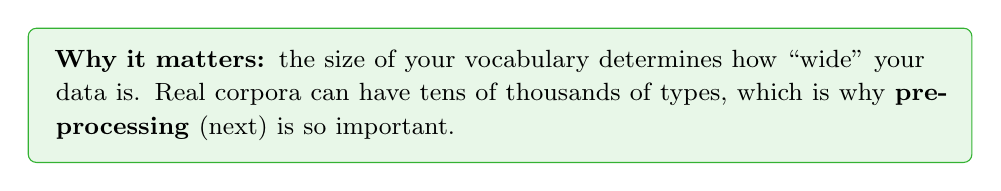
\begin{tikzpicture}
  \node[fill=lightgreen, draw=wurgreen, rounded corners=3pt,
        inner xsep=10pt, inner ysep=8pt, text width=\textwidth-24pt]{%
    {\small\textbf{Why it matters:} the size of your vocabulary determines how
    ``wide'' your data is. Real corpora can have tens of thousands of types,
    which is why \textbf{preprocessing} (next) is so important.}};
\end{tikzpicture}
\end{frame}

% ── SLIDE 6: Prerequisites - preprocessing mindset ───────────────────────────
\begin{frame}{Prerequisite Concepts (3): The Preprocessing Mindset}
\vspace{0.2cm}
{\small Before counting, we usually \textbf{clean and normalize} text.
Each choice is a \textbf{modeling decision}, not just housekeeping ---
it changes what your numbers mean.}

\bigskip
\begin{columns}[t]
  \column{0.48\textwidth}
  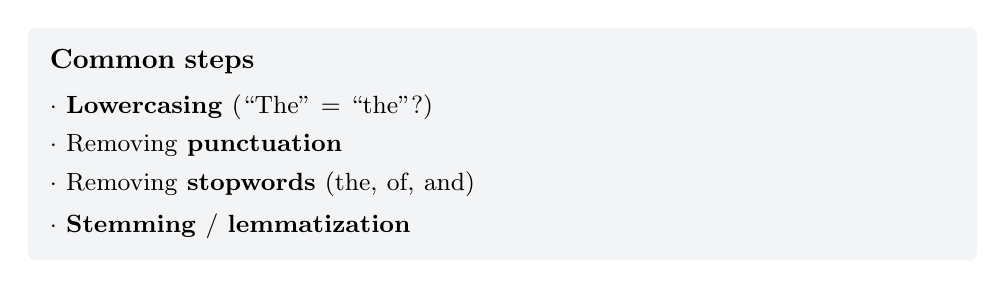
\begin{tikzpicture}
    \node[fill=lightgray, rounded corners=3pt,
          inner xsep=8pt, inner ysep=8pt, text width=\columnwidth-18pt]{%
      \textbf{Common steps}\\[5pt]
      {\small
      $\cdot$ \textbf{Lowercasing} (``The'' = ``the''?)\\[3pt]
      $\cdot$ Removing \textbf{punctuation}\\[3pt]
      $\cdot$ Removing \textbf{stopwords} (the, of, and)\\[3pt]
      $\cdot$ \textbf{Stemming} / \textbf{lemmatization}}};
  \end{tikzpicture}

  \column{0.48\textwidth}
  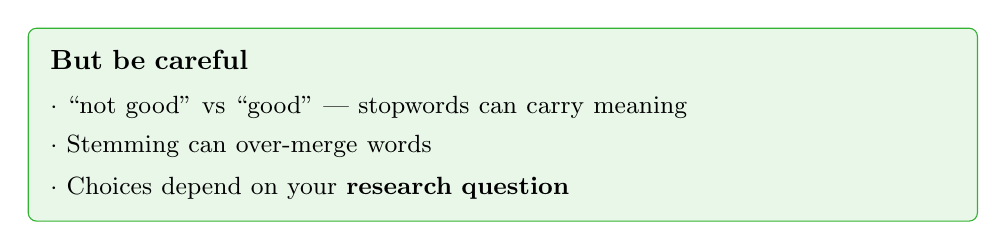
\begin{tikzpicture}
    \node[fill=lightgreen, draw=wurgreen, rounded corners=3pt,
          inner xsep=8pt, inner ysep=8pt, text width=\columnwidth-18pt]{%
      \textbf{But be careful}\\[5pt]
      {\small
      $\cdot$ ``not good'' vs ``good'' --- stopwords can carry meaning\\[3pt]
      $\cdot$ Stemming can over-merge words\\[3pt]
      $\cdot$ Choices depend on your \textbf{research question}}};
  \end{tikzpicture}
\end{columns}

\medskip
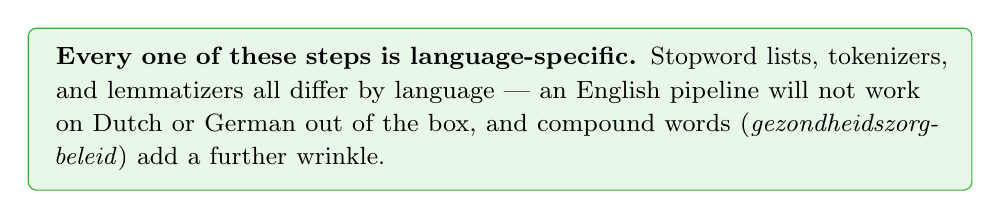
\begin{tikzpicture}
  \node[fill=lightgreen, draw=wurgreen, rounded corners=3pt,
        inner xsep=10pt, inner ysep=7pt, text width=\textwidth-24pt]{%
    {\small \textbf{Every one of these steps is language-specific.} Stopword lists, tokenizers,
    and lemmatizers all differ by language --- an English pipeline will not work on Dutch or
    German out of the box, and compound words (\textit{gezondheidszorgbeleid}) add a further
    wrinkle.}};
\end{tikzpicture}
\end{frame}

% ── SLIDE 7: DTM concept ─────────────────────────────────────────────────────
\begin{frame}{The Document-Term Matrix (DTM)}
\vspace{0.2cm}
{\small The \textbf{document-term matrix} is where it all comes together.
Rows are \textbf{documents}, columns are \textbf{terms} (your vocabulary),
and each cell holds a \textbf{count}: how often that term appears in that document.}

\bigskip
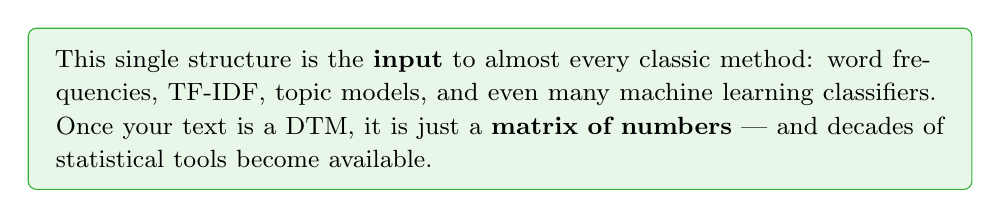
\begin{tikzpicture}
  \node[fill=lightgreen, draw=wurgreen, rounded corners=3pt,
        inner xsep=10pt, inner ysep=8pt, text width=\textwidth-24pt]{%
    {\small This single structure is the \textbf{input} to almost every classic
    method: word frequencies, TF-IDF, topic models, and even many machine
    learning classifiers. Once your text is a DTM, it is just a \textbf{matrix of
    numbers} --- and decades of statistical tools become available.}};
\end{tikzpicture}

\bigskip
{\small\textcolor{midgray}{\textit{Let's build one by hand.}}}
\end{frame}

% ── SLIDE 8: DTM worked example ──────────────────────────────────────────────
\begin{frame}{Worked Example: Building a DTM}
\vspace{0.2cm}
{\small Three short ``documents'':}
\smallskip

{\small
\textbf{D1:} the cat sat \quad
\textbf{D2:} the dog sat \quad
\textbf{D3:} the cat ran}

\bigskip
\begin{center}
\setlength{\arrayrulewidth}{0.3pt}
\renewcommand{\arraystretch}{1.4}
\begin{tabular}{l|ccccc}
  & \textbf{the} & \textbf{cat} & \textbf{sat} & \textbf{dog} & \textbf{ran} \\
\hline
\textbf{D1} & 1 & 1 & 1 & 0 & 0 \\
\textbf{D2} & 1 & 0 & 1 & 1 & 0 \\
\textbf{D3} & 1 & 1 & 0 & 0 & 1 \\
\end{tabular}
\end{center}

\bigskip
{\small Each \textbf{row} is a document as a vector of counts. Each \textbf{column}
is a term across all documents. That is the entire idea --- and everything in the
coming sessions builds on this simple table.}
\end{frame}

% ── SLIDE 8b: TF-IDF motivation ──────────────────────────────────────────────
\begin{frame}{A Problem with Raw Counts}
\vspace{0.2cm}
{\small Look again at the DTM. The word \textbf{``the''} appears in \textbf{every}
document --- so it is useless for telling them apart. Raw counts give \textbf{common
words too much weight} and \textbf{distinctive words too little}.}

\bigskip
\begin{columns}[T]
  \column{0.48\textwidth}
  \vspace{0pt}
  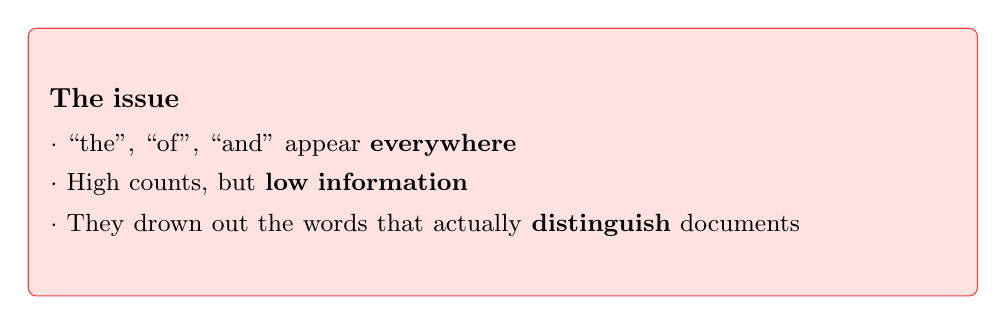
\begin{tikzpicture}
    \node[fill=warnred, draw=warnborder, rounded corners=3pt,
          inner xsep=8pt, inner ysep=8pt, text width=\columnwidth-18pt, minimum height=3.4cm]{%
      \textbf{The issue}\\[5pt]
      {\small
      $\cdot$ ``the'', ``of'', ``and'' appear \textbf{everywhere}\\[3pt]
      $\cdot$ High counts, but \textbf{low information}\\[3pt]
      $\cdot$ They drown out the words that actually \textbf{distinguish} documents}};
  \end{tikzpicture}

  \column{0.48\textwidth}
  \vspace{0pt}
  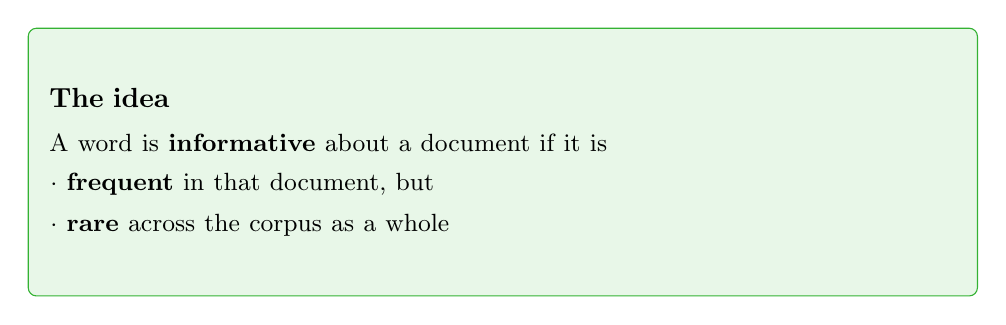
\begin{tikzpicture}
    \node[fill=lightgreen, draw=wurgreen, rounded corners=3pt,
          inner xsep=8pt, inner ysep=8pt, text width=\columnwidth-18pt, minimum height=3.4cm]{%
      \textbf{The idea}\\[5pt]
      {\small
      A word is \textbf{informative} about a document if it is\\[3pt]
      $\cdot$ \textbf{frequent} in that document, but\\[3pt]
      $\cdot$ \textbf{rare} across the corpus as a whole}};
  \end{tikzpicture}
\end{columns}

\medskip
{\small\textcolor{midgray}{\textit{This is exactly what \textbf{TF-IDF} captures.}}}
\end{frame}

% ── SLIDE 8c: TF-IDF explained ───────────────────────────────────────────────
\begin{frame}{TF-IDF: Term Frequency $\times$ Inverse Document Frequency}
\vspace{0.2cm}
{\small \textbf{TF-IDF} reweights each cell of the DTM by multiplying two quantities:}

\medskip
\begin{columns}[T]
  \column{0.48\textwidth}
  \vspace{0pt}
  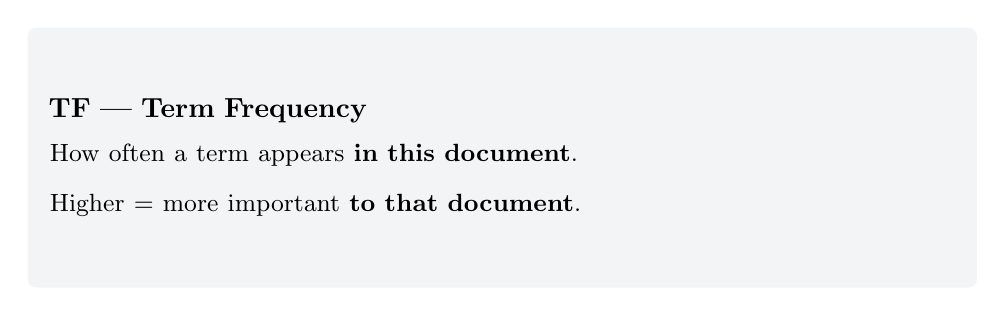
\begin{tikzpicture}
    \node[fill=lightgray, rounded corners=3pt,
          inner xsep=8pt, inner ysep=8pt, text width=\columnwidth-18pt, minimum height=3.3cm]{%
      \textbf{TF --- Term Frequency}\\[5pt]
      {\small How often a term appears \textbf{in this document}.\\[6pt]
      Higher = more important \textbf{to that document}.}};
  \end{tikzpicture}

  \column{0.48\textwidth}
  \vspace{0pt}
  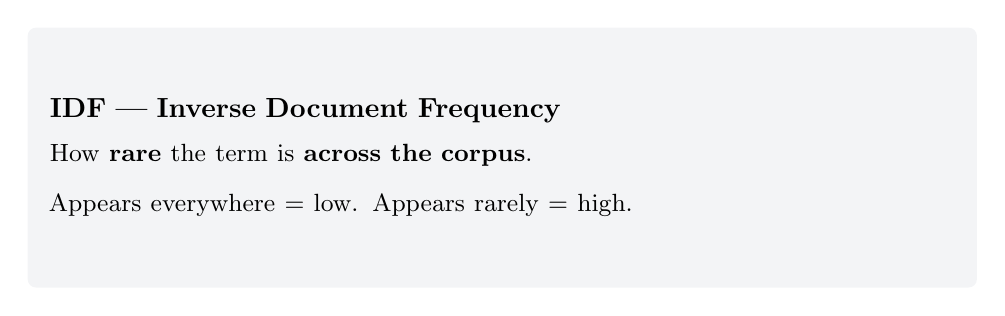
\begin{tikzpicture}
    \node[fill=lightgray, rounded corners=3pt,
          inner xsep=8pt, inner ysep=8pt, text width=\columnwidth-18pt, minimum height=3.3cm]{%
      \textbf{IDF --- Inverse Document Frequency}\\[5pt]
      {\small How \textbf{rare} the term is \textbf{across the corpus}.\\[6pt]
      Appears everywhere = low. Appears rarely = high.}};
  \end{tikzpicture}
\end{columns}

\medskip
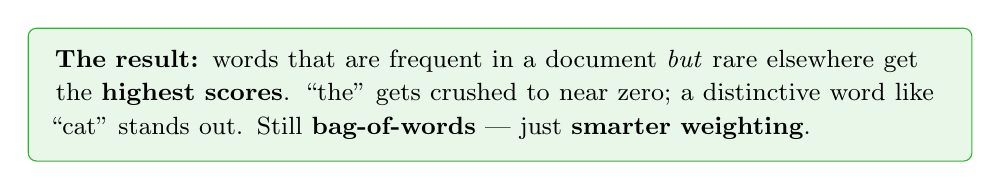
\begin{tikzpicture}
  \node[fill=lightgreen, draw=wurgreen, rounded corners=3pt,
        inner xsep=10pt, inner ysep=8pt, text width=\textwidth-24pt]{%
    {\small \textbf{The result:} words that are frequent in a document \emph{but} rare
    elsewhere get the \textbf{highest scores}. ``the'' gets crushed to near zero;
    a distinctive word like ``cat'' stands out. Still \textbf{bag-of-words} --- just
    \textbf{smarter weighting}.}};
\end{tikzpicture}
\end{frame}

% ── SLIDE 9: Recap ───────────────────────────────────────────────────────────
\begin{frame}{Before We Start Coding}
\vspace{0.3cm}
{\small You now have the vocabulary you need. Make sure these feel clear:}

\bigskip
\begin{columns}[t]
  \column{0.48\textwidth}
  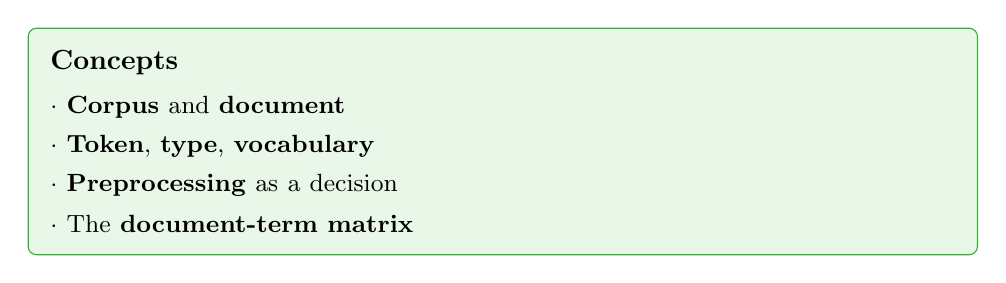
\begin{tikzpicture}
    \node[fill=lightgreen, draw=wurgreen, rounded corners=3pt,
          inner xsep=8pt, inner ysep=8pt, text width=\columnwidth-18pt]{%
      \textbf{Concepts}\\[5pt]
      {\small
      $\cdot$ \textbf{Corpus} and \textbf{document}\\[3pt]
      $\cdot$ \textbf{Token}, \textbf{type}, \textbf{vocabulary}\\[3pt]
      $\cdot$ \textbf{Preprocessing} as a decision\\[3pt]
      $\cdot$ The \textbf{document-term matrix}}};
  \end{tikzpicture}

  \column{0.48\textwidth}
  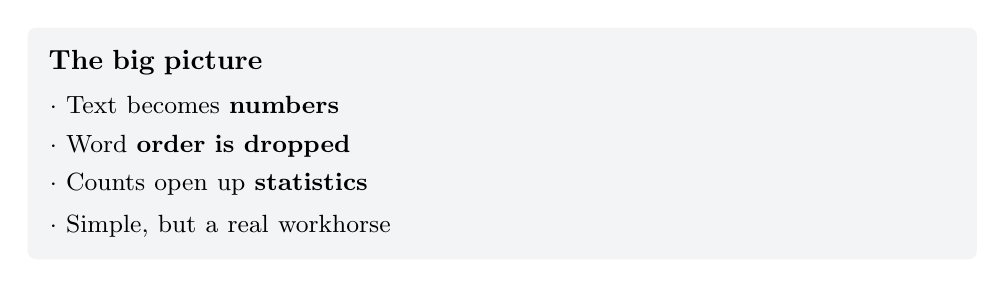
\begin{tikzpicture}
    \node[fill=lightgray, rounded corners=3pt,
          inner xsep=8pt, inner ysep=8pt, text width=\columnwidth-18pt]{%
      \textbf{The big picture}\\[5pt]
      {\small
      $\cdot$ Text becomes \textbf{numbers}\\[3pt]
      $\cdot$ Word \textbf{order is dropped}\\[3pt]
      $\cdot$ Counts open up \textbf{statistics}\\[3pt]
      $\cdot$ Simple, but a real workhorse}};
  \end{tikzpicture}
\end{columns}

\bigskip
{\small\textcolor{midgray}{\textit{Next: we build these matrices in Python and put them to work.}}}
\end{frame}

\end{document}
